\documentclass[a4paper,12pt]{report}

\usepackage{alltt, fancyvrb, url}
\usepackage{graphicx}
\usepackage[utf8]{inputenc}
\usepackage{float}
\usepackage{hyperref}

% Questo commentalo se vuoi scrivere in inglese.
\usepackage[italian]{babel}

\usepackage[italian]{cleveref}

\title{Relazione per \\``Programmazione ad Oggetti'' \\ \\Progetto ''Unibo-td''}

\author{Aurora Francesco, Casali Marco, Murvai Cristina, Pulga Luca}
\date{04 luglio 2024}


\begin{document}

\maketitle

\tableofcontents

\chapter{Analisi}

Questo documento fornisce una panoramica dei requisiti fondamentali per lo sviluppo del gioco Tower-Defense ispirato a Bloons TD. I requisiti tecnici dettagliati e le specifiche implementative saranno trattati in fasi successive del processo di sviluppo, mantenendo il focus sul comportamento e le funzionalità dell'applicazione.

\begin{figure}[H]
    \centering
    \includegraphics[width=1\textwidth]{intro.jpg}
    \caption{Schermata di un tipico gioco Tower-Defense}
    \label{fig:enter-label}
\end{figure}


\section{Requisiti}

L'obiettivo del presente documento è definire i requisiti dell'applicazione per il gioco di tipo Tower-Defense ispirato a Bloons TD. Questo gioco sarà progettato per offrire un'esperienza coinvolgente simile al gioco di riferimento, adattata alle specifiche del progetto.

\subsection*{Requisiti funzionali}
\begin{itemize}
	\item Un gioco di tipo Tower Defense è un genere in cui i giocatori devono posizionare torri strategiche lungo un percorso per fermare onde di nemici. Le torri, ciascuna con abilità specifiche, devono essere posizionate strategicamente per prevenire che i nemici raggiungano un punto finale, solitamente la base o un obiettivo.
	\item Deve essere possibile avviare un nuovo gioco e visualizzare informazioni essenziali come punteggi e stato del gioco.
	\item Dividere il gioco in round con difficoltà incrementale.
	\item Creare una mappa giocabile con percorsi definiti per i nemici.
	\item Gli utenti devono poter piazzare diverse torri lungo il percordo di gioco per difendersi dai nemici.
	\item Le torri devono essere posizionabili in punti specifici del campo.
	\item Ogni difesa deve avere esattamente una arma utilizzabile.
	\item Deve essere possibile avviare un nuovo gioco e visualizzare informazioni essenziali come punteggi e stato del gioco.
	\item Gestire le interazioni tra i nemici e le difese, inclusi attacchi e difese delle torri.
	\item Gestire un sistema di vite limitate per i giocatori; il gioco termina quando le vite si esauriscono.
	\item Implementare un sistema di gestione economica per guadagnare e spendere monete nelle difese.
\end{itemize}

\subsection*{Requisiti non funzionali}
\begin{itemize}
	\item Garantire fluidità del gioco su diverse piattaforme, con un'attenzione particolare alla velocità di caricamento dei livelli e all'ottimizzazione generale.
	\item Assicurare che il gioco sia compatibile con dispositivi desktop supportando almeno le versioni recenti dei principali sistemi operativi (windows, linux, macos).
\end{itemize}

\section{Analisi e modello del dominio}

Unibo TD avrà più entità che dovranno collaborare tra loro.

\subsection*{Gestione delle difese}
\begin{itemize}
Il gioco sarà costituito da una mappa. All'interno della mappa saranno presenti delle celle edificabili su cui poter posizionare le proprie difese (\textit{torri}). 
Le difese sono le unità incaricate a proteggere il punto terminale della mappa. Queste saranno quindi in grado di infliggere danni ai nemici attraverso specifiche logiche di targettamento e di attacco. Ogni tipologia difesa possiederà certe statistiche per poter garantire maggiore eterogeneità al gioco. Per costruire una difesa sarà necessaria una certa quantità di denaro, acquisibile tramite l'eliminazione di nemici nei vari round. Ogni difesa oltre ad avere relative speficifiche e caratteristiche, fra queste figurano anche le \textit{armi} a disposizione di ogni torre, le quali gestiscono la \textit{frequenza} di sparo dei \textit{proiettili} per arrecare danno ai nemici. Ogni proiettile sparato da una determinata torre con una determinata arma, dispone di un certo danno. Ogni qualvolta una difesa sconfigge un nemico, verrà accreditato al \textbf{player} il denaro relativo al nemico sconfitto. Due feature interessanti sarebbero la rimozione e il riposizionamento delle difese sulla mappa nei punti permessi. Queste purtroppo non potranno essere effettuate all’interno del monte ore previsto e conseguentemente si rimanda tale feature in futuro.
\end{itemize}

\chapter{Design}

\section{Architettura}

L'architettura dell'applicazione sviluppata si basa sul modello architetturale MVC (Model-Controller-View). Il Model, una volta avviato dal Controller, esternalizza e gestisce in modo trasparente la logica tramite il defense manager e l'enemy manager, i quali si occupano di aspetti diversi del gioco, come i nemici e le difese. Il Controller funge da intermediario tra Model e View, limitando l'accesso diretto al Model e fornendo solo oggetti di trasferimento dati. Ciò significa che gli altri componenti dell'applicazione, come la View, possono accedere solo a una rappresentazione immutabile dei dati nel Model, garantendo un maggiore controllo sull'integrità dei dati. Di conseguenza, l'implementazione della View, così come è stata definita, è facilmente sostituibile poiché non dipende dalle classi sottostanti.
\begin{figure}
    \centering
    
\includegraphics[width=0.5\linewidth]{todo.jpg}
    \caption{Architettura MVC}
    \label{fig:enter-label}
\end{figure}
\section{Design dettagliato}
\textbf{Luca Pulga}
\subsection{Gestione delle difese}

\textbf{Problema}:
Si vuole gestire in maniera scalabile le varie entità presenti all'interno del gioco, come le difese (torri, armi, proiettili) e i nemici, evitando l'eccessiva scrittura di codice duplicato.

\textbf{Soluzione}:
E' possibile suddividere le varie caratteristiche delle varie entità in sotto-entità, in modo da attribuire le relative proprietà ad ogni tipologia di entità che è presente
o che potrà essere presente in futuro, rendendo la struttura scalabile. Sono state realizzate interfacce e classi astratte, a cui sono state delegate le assegnazioni delle varie proprietà, fornendo la condivisione del codice comune e contratti parziali, implementabili dalle sottoclassi.
Un'ulteriore soluzione poteva essere quella di utilizzare solo interfacce e come implementazione di esse utilizzare i record, in quanto fornirebbero un modo decisamente più coinciso per dichiarare classi immutabili ed eliminerebbero molta della verbosità associata alle classi standard.

\begin{figure}[H]
    \centering
    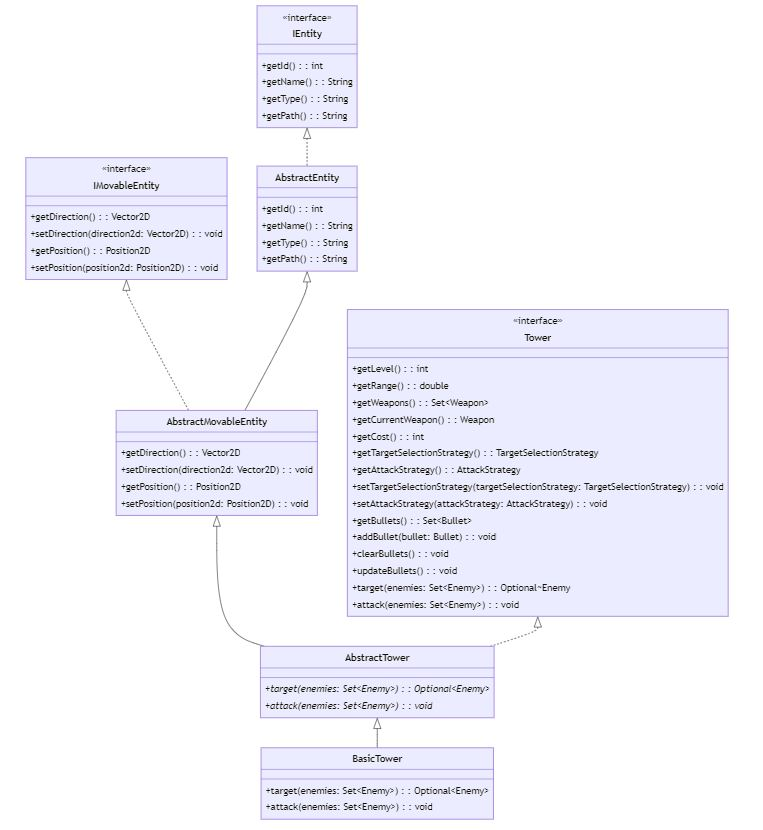
\includegraphics[width=1.2\linewidth]{defense_model.JPG}
    \caption{Modello per la gestione delle entità.}
    \label{fig:defense-model}
\end{figure}

\vspace{15mm}

\textbf{Problema}:
Disporre di un oggetto in grado di poter creare qualsiasi tipo di entità, centralizzando la parte di creazione degli oggetti che verranno caricati e successivamente utilizzati durante il gioco.

\textbf{Soluzione}:
Si utilizza il \textit{Factory Method Pattern} in modo da sfruttare la sua capacità di separare la costruzione degli oggetti dal loro utilizzo. Dunque questa separazione ci consente di avere una maggiore flessibilità e modularità del codice, rendendolo più facile da mantenere e aggiornare anche introducendo in futuro nuove entità o separare in sotto-entità quelle già esistenti. 
La \textit{Factory} provvederà a leggere i files json all'interno di specifiche cartelle per caricare
le entità, come le \textit{torri}, che saranno poi successivamente gestite dal \textit{Defense Manager}.
\begin{figure}[H]
    \centering
    
\includegraphics[width=0.8\linewidth]{todo.jpg}
    \caption{Factory Method Pattern per il caricamento delle entità.}
    \label{fig:entity-factory-method}
\end{figure}
\vspace{25mm}

\textbf{Problema}:
Gestione delle istanze delle torri senza avere un'entità centralizzata.
\textbf{Soluzione}:
La soluzione prevedere l'implementazione di un Defense Manager in grado di gestire le entità difesa. Questa soluzione centralizzata permette di gestire all'interno di un unica classe tutte le entità difesa, fornendo anche un modo comodo all'esterno per ottenere informazioni con altri oggetti.

\begin{figure}[H]
    \centering
    
\includegraphics[width=0.8\linewidth]{todo.jpg}
    \caption{Defense Manager per la gestione delle difese.}
    \label{fig:defense-manager}
\end{figure}

\vspace{50mm}
\textbf{Problema}:
Gestione di varie tipologie di entità in tempo reale come torri, proiettili, nemici e tutte le varie entità che potrebbero essere introdotte in futuro che hanno necessità di reagire a certi eventi.
\textbf{Soluzione}:
A livello di difese, si sottoscrive il Defense Manager all'Observer, il quale consente di definire un meccanismo di sottoscrizione per notificare a più oggetti gli eventi che accadono all'oggetto che stanno osservando, tutto ciò rispettando il principio Open/Closed, migliorando così la modularità e la manutenibilità del codice.

\begin{figure}[H]
    \centering
    
\includegraphics[width=0.8\linewidth]{todo.jpg}
    \caption{Figura 2.5: Defense Manager e Observer.}
    \label{fig:defense-observer}
\end{figure}
\vspace{50mm}
\textbf{Problema}:
Implementazione di diverse tipologie di targettamento dei nemici da parte delle torri a seconda della loro tipologia.
\textbf{Soluzione}:
Si implementa lo Strategy Pattern, in questo modo il contesto diventa indipendente dalle strategie concrete di targettamento dei nemici, per cui è possibile aggiungere/modificare gli algoritmi di targettamento senza modificare il codice all'interno delle varie classi che potrebbero implementare la relativa strategia di attacco.

\begin{figure}[H]
    \centering
    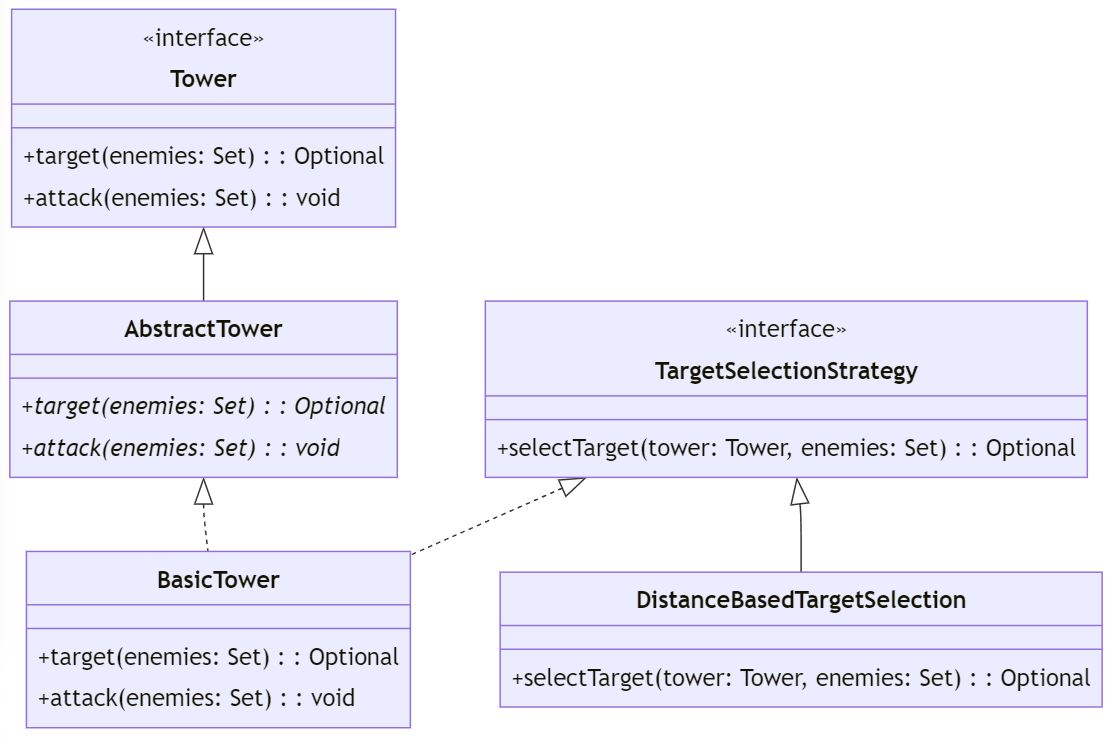
\includegraphics[width=0.8\linewidth]{defense_target.JPG}
    \caption{Pattern Strategy per targettamento dei nemici.}
    \label{fig:defense_target}
\end{figure}



\textbf{Problema}:
Implementazione di diverse tipologie di attacchi verso i nemici da parte delle torri a seconda della loro tipologia.
\textbf{Soluzione}:
Si implementa lo Strategy Pattern, in questo modo il contesto diventa indipendente dalle strategie concrete di attacco verso i nemici, per cui è possibile aggiungere/modificare gli algoritmi di attacco senza modificare il codice all'interno delle varie classi che potrebbero implementare la relativa strategia di attacco.

\begin{figure}[H]
    \centering
    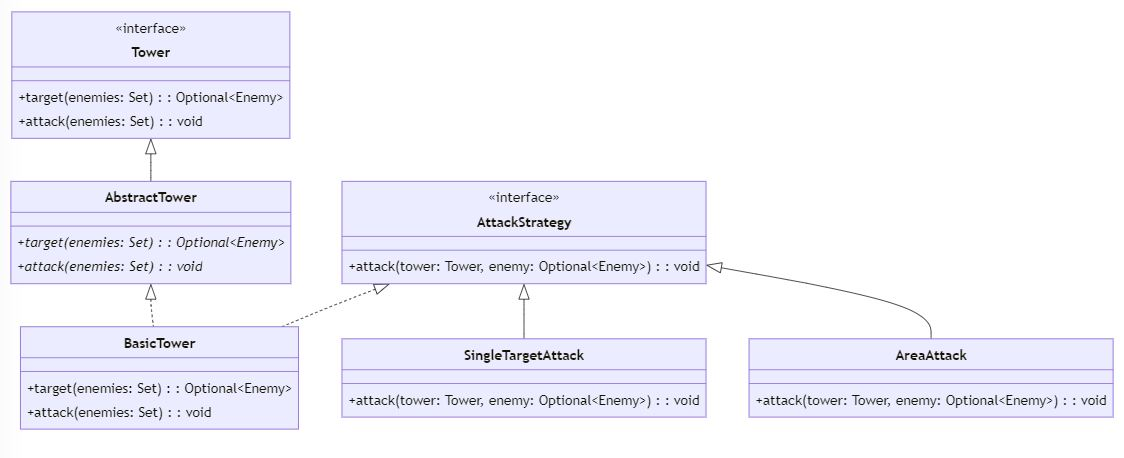
\includegraphics[width=0.8\linewidth]{defense_attack.JPG}
    \caption{Pattern Strategy per attacco ai nemici.}
    \label{fig:defense_attack}
\end{figure}


\chapter{Sviluppo}
\section{Testing automatizzato}
Per verificare il corretto funzionamento del gioco Tower-Defense, sono stati creati appositi test automatizzati utilizzando JUnit. 
I test automatizzati sono necessari per poter testare se le logiche pensate durante la fase analisi, di progettazione e di implementazione del Model, e delle classi affini di utility, sono funzionanti.

\begin{itemize}
    \item \textit{\textbf{TestBasicTower}:} Test automatizzato per garantire la correttezza dei metodi di get e set delle difese torri per poter gestire durante il gioco le sue proprietà.
    \item \textit{\textbf{TestBulletImpl}:} Test automatizzato per garantire la correttezza dei metodi di get e set della posizione e direzione del proiettile, fondamentale per la gestione grafica del gioco.
    \item \textit{\textbf{TestDefenseFactory}:} Test automatizzato per garantire la correttezza di lettura da file json delle entità torri attraverso l'utilizzo della \ref{fig:entity-factory-method}EntityFactory
    \item \textit{\textbf{TestTargetStrategy}:} Test automatizzato per garantire la correttezza dei calcoli effettuati durante la fase di targettamento di nemici da parte delle torri.
\end{itemize}

\section{Note di sviluppo}
\chapter{Luca Pulga}

\subsubsection{Utilizzo di Optional}
Utilizzati in vari punti. Un esempio: 
\url{https://github.com/PulgaLuca/OOP23-unibo-td/blob/12d7eec3c7e4b474e6f315461642e1c6a2d6c693/src/main/java/it/unibo/model/entities/defense/tower/target/DistanceBasedTargetSelection.java#L24}

\subsubsection{Utilizzo di generici}
\url{https://github.com/PulgaLuca/OOP23-unibo-td/blob/12d7eec3c7e4b474e6f315461642e1c6a2d6c693/src/main/java/it/unibo/model/entities/EntityFactoryImpl.java#L40}

\subsubsection{Utilizzo di lambda expressions}
Utilizzate in vari punti. Un esempio:  
\url{https://github.com/PulgaLuca/OOP23-unibo-td/blame/12d7eec3c7e4b474e6f315461642e1c6a2d6c693/src/main/java/it/unibo/model/entities/defense/manager/DefenseManagerImpl.java#L96}

\subsubsection{Utilizzo della libreria SLF4J}
Utilizzata in vari punti. Un esempio:  
\url{https://github.com/PulgaLuca/OOP23-unibo-td/blame/12d7eec3c7e4b474e6f315461642e1c6a2d6c693/src/main/java/it/unibo/model/entities/defense/manager/DefenseManagerImpl.java#L29C43-L29C43}

\subsubsection{Utilizzo della libreria Jackson per interazione con file JSON}
Un esempio:  
\url{https://github.com/PulgaLuca/OOP23-unibo-td/blob/12d7eec3c7e4b474e6f315461642e1c6a2d6c693/src/main/java/it/unibo/model/entities/EntityFactoryImpl.java#L66}


\chapter{Commenti finali}
\subsubsection{Luca Pulga}
Prendere parte a questo progetto è stata un'attività non semplicissima ma decisamente formativa, soprattutto in ottica futura.
La progettazione della parte difensiva del gioco ricopre un ruolo massivo dell'applicazione e ho cercato non solo di cimentarmi nella mia parte di difese, ma anche nel cercare una generalizzazione relativamente alle varie tipologie di entità presenti nel gioco. La soluzione adottata rende estendibile il codice in caso di futuri sviluppi, attraverso l'astrazione delle entità e all'utilizzo di Design Patterns fondamentali per rendere il codice maggiormente leggibile e scalabile. Purtroppo non sono riuscito a sfruttare a pieno la programmazione funzionale e altre tecniche di programmazione illustrate durante il corso, che mi sarebbe interessato implementare e progettare, ma che porto ora con me nel mio bagaglio formativo. Non sono totalmente appagato dalla UX/UI per la parte di difese per quanto riguarda il posizionamento delle torri ma generalmente credo di essere riuscito a creare comunque applicativo giocabile. Infine direi che sono comunque soddisfatto non solo di aver acquisito nuove competenze ma anche di aver conosciuto persone nuove e di aver lavorato in un team per me nuovo.


\appendix
\chapter{Guida utente}

Capitolo in cui si spiega come utilizzare il software. Nel caso in cui il suo uso sia del tutto
banale, tale capitolo può essere omesso.
%
A tal riguardo, si fa presente agli studenti che i docenti non hanno mai utilizzato il software
prima, per cui aspetti che sembrano del tutto banali a chi ha sviluppato l'applicazione possono non
esserlo per chi la usa per la prima volta.
%
Se, ad esempio, per cominciare una partita con un videogioco è necessario premere la barra
spaziatrice, o il tasto ``P'', è necessario che gli studenti lo segnalino.

\subsection*{Elementi positivi}

\begin{itemize}
 \item Si istruisce in modo semplice l'utente sull'uso dell'applicazione, eventualmente facendo uso di schermate e descrizioni.
\end{itemize}

\subsection*{Elementi negativi}
\begin{itemize}
 \item Si descrivono in modo eccessivamente minuzioso tutte le caratteristiche, anche minori, del software in oggetto.
 \item Manca una descrizione che consenta ad un utente qualunque di utilizzare almeno le funzionalità primarie dell'applicativo.
\end{itemize}

\chapter{Esercitazioni di laboratorio}

\section*{Esempio}

\subsection{paolino.paperino@studio.unibo.it}

\begin{itemize}
 \item Laboratorio 04: \url{https://virtuale.unibo.it/mod/forum/discuss.php?d=12345#p123456}
\end{itemize}

\bibliographystyle{alpha}
\bibliography{13-template}

\end{document}
